\documentclass{article}
\usepackage[utf8]{inputenc}
\usepackage{amsmath}
\usepackage{graphicx}
\usepackage{listings}
\usepackage{natbib}
\usepackage{tikz}
\usepackage{gensymb}
\usetikzlibrary{arrows,decorations.markings,decorations.pathmorphing,patterns}
\newcommand\centerofmass{%
    \tikz[radius=0.4em] {%
        \fill (0,0) -- ++(0.4em,0) arc [start angle=0,end angle=90] -- ++(0,-0.8em) arc [start angle=270, end angle=180];%
        \draw (0,0) circle;%
    }%
}

\title{CDT Documentation}
\author{David Eade}
\date{September 4, 2020}

\begin{document}

\maketitle

\tableofcontents

\section{Introduction}
For the past several years, I've been designing catapults using a mish-mash of stress analysis tools, rigid body dynamics tools, and my own half-baked code to fill in the gaps. The dearth of purpose-built catapult design tools makes the hobby difficult to access for most people without a solid mechanical engineering background or a lot of time and money to spend on failed prototypes. Although the CDT does not fully solve the accessibility problem yet, mainly owing to the absence of an arm stress analysis tool, I hope it will open up the hobby to a wider audience. The design and construction of catapults is a rich and rewarding pastime, with many low hanging fruit still waiting to be picked, and I look forward to having more people to share it with.\par
The Catapult Design Tool (CDT) is intended to provide a quick, user friendly means of estimating catapult dynamics for use in feasibility studies and tuning, and finding loading states for the stress analysis work involved in arm design. The backend code is readily extensible such that the advanced user can add everything from custom torque functions and diagnostics, to upgrades to the core of the dynamics solver itself. It is NOT intended as a fully detailed simulation, and the user is advised to be aware of its capabilities and limitations.\par
The CDT can be used in two ways: Through the included GUI, or by directly using the functions provided by the Python package. This guide is mainly directed at users of the GUI. Advanced users should have little trouble inspecting the GUI code to see which functions in the package do the simulation and optimization.

\section{The Model}
The CDT models a catapult as a forced double pendulum with rigid links and no air resistance.  The forcing function is torque as a function of arm angle, and while there are many means of generating this function available to the user, the end result is always a 10th-order polynomial $\tau(\theta)$. The torque source has no dynamics of its own.\\


\subsection{Dynamics Assembly Parameters} \label{Dynamics Assembly Parameters}
\begin{tikzpicture}
\coordinate (arm tip) at (-3,-5.19616);
\draw[gray, thick] (0,0) -- node[above left] {$L_a$} (arm tip);
\filldraw[black] (arm tip) circle (2pt);;
\draw[gray, thick, dashed, ->] (arm tip) arc(240:210:6cm) node[above, align=center] {throwing\\direction};
\draw[gray, thick, ->] (arm tip) -- (-3.5, -6.062177826) node[anchor=north] {$x_A$};
\draw[gray, thick, ->] (arm tip) -- (-2.1339746, -5.69616) node[anchor=north] {$y_A$};
\node[below right] at (-3,-6.1) {tip frame};
\node at (-1,-1.73205){$\centerofmass$};
\node at (-0.6,-1.73205){$m_b$};

\draw[gray, thick] (-3, -5.19616) -- node[below] {$L_s$} (4.8784,-6.585338);
\filldraw[black] (4.8784,-6.585338) circle (3pt) node[anchor=west] {$m_p$};

\draw[gray, thick, dashed] (0,0) -- (0,-2);
\draw[gray, thick, dashed] (0,0) -- (1,1.73205); 
\draw[decoration={markings,mark=at position 1 with {\arrow[scale=2,>=stealth]{>}}},postaction={decorate}] (0,-1) arc(-90:60:1cm);
\node[](theta) at (0.4, -0.2){$\theta$}; % theta label
\draw[decoration={markings,mark=at position 1 with {\arrow[scale=2,>=stealth]{>}}},postaction={decorate}] (-2.5, -4.330127) arc(60:-10:1cm);
\node[](psi) at (-2.45, -4.9){$\psi$}; % psi label
\filldraw[black] (0,0) circle (2pt) node[above left] {(0, 0)}; %origin
\coordinate (BFO) at (2,-3);
\draw[gray, thick, ->] (BFO) -- (3,-3) node[anchor=west] {x};
\draw[gray, thick, ->] (BFO) -- (2,-2) node[anchor=south] {y}; %coordinate system
\node[below] at (BFO) {base frame};

\end{tikzpicture}

\begin{description}
\item $\rho_p$: linear density of sling
\item $g$: gravitational acceleration (default 9.8)
\item $r_c$: distance from pivot to arm centre of mass
\item $I_A$: rotational inertia of arm about axis of rotation
\item $m_b$: arm mass
\item $m_p$: projectile mass
\item $L_a$: arm length
\item $L_s$: sling length
\end{description}

\subsection{State Variables}
The configuration of the system is fully specified by two generalized coordinates, $\theta$ and $\psi$, corresponding to the angle of the arm relative to the base and the angle of the sling relative to the arm. The state of the system is thus $\mathbf{y} = (\theta, \dot{\theta}, \psi, \dot{\psi})^\top$. By writing the kinetic and potential energy of the system in terms of the generalized coordinates we can find the Lagrangian, after which applying the Euler-Lagrange equation yields the differential equations describing the motion. These are rather bulky, and have been omitted for brevity. The interested reader can find them in dynlib.c.

\subsection{Simulation} \label{Simulation}
Two main cases are handled by the dynamics solver: the standard catapult depicted above, and one where a mechanical stop ("platform") prevents $\psi$ from decreasing below its initial value. In the second case, the entire assembly initially rotates together, with no change in $\psi$, until the force due to angular rotation trying to lift the projectile off the platform exceeds the force due to angular acceleration trying to hold it down. This entails transitioning between dynamics models mid-throw.\par

The solver uses the RK4 method to integrate the ODEs describing the system's dynamics. As such, it is necessary for the user to specify a time step. Standard considerations for numerical convergence apply, although in the range of interest for practical trebuchet design the equations are numerically well-behaved. Something on the order of 1000 time steps is typically sufficient for good convergence. When transitions between models are present or a stop condition is reached, a bisection search is used to precisely determine the transition time. This means that solutions using the platform option will typically have a single short time step somewhere in the middle. \par


\subsection{Torque Source}
Despite the plethora of options available to the user in specifying aspects of the torque function, internally it is represented by only twelve parameters:
\[\tau(\theta) = m\tau_1(\theta)\]
\[\tau_1(\theta) = c_0 + c_1\theta + c_2\theta^2 + \ldots + c_{10}\theta^{10}\]
where
\[m = \begin{cases} k_w &(\dot{\theta}>0)\oplus(\tau_1<0)\\
1 & \mbox{else } \end{cases}\]
Which is to say the value of the polynomial is multiplied by $k_w$ if the arm is backdriving or the torque is below zero, but not both. The astute reader may find themselves wondering what that has to do with the price of tea in China.

\subsubsection{Torque Source Sign Convention}
The torque applied in the simulation is the \emph{negative} of the value of $\tau$ calculated in the above equation. %use numbered equations instead
This was done so that the intuitive approach of a positive torque causing the machine to throw would work, but is regrettably confusing for those who correctly expect a positive torque to cause a positive angular acceleration. So, $\dot{\theta} > 0$ corresponds to the arm rotating in the "wrong" direction, and $\tau_1 < 0$ corresponds to the torque source driving the arm in the "wrong" direction. Thus, if we imagine that a linear actuator of some sort is creating the torque, we see that $m=1$ if the actuator is contracting, and $m=k_w$ if the actuator is extending.

\subsubsection{Hysteresis}
Rubber bands are an excellent and fairly common energy source for catapults, and they pull roughly twice as hard while being extended as they do while contracting. The value of $k_w$ is simply the ratio between the force while extending and the force while contracting. If the force during extension is higher, $k_w > 1$. Although 2 is a good approximate value, it is recommended that the user tests the rubber they intend to use under conditions representative of their application for best accuracy.

\subsection{Limitations}
As mentioned in the introduction, the CDT is not intended to provide a highly accurate, realistic dynamical model. For this purpose, rigid body dynamics or explicit dynamics tools are recommended. The CDT also does not provide stress analysis tools, which are a necessity when designing higher performance machines with complicated arm geometries. At low speeds, simple geometries that are amenable to hand calculation will often suffice. 

\subsubsection{Dynamics Model}
The CDT dynamics model behaves differently than a real catapult in three important ways:
\begin{enumerate}
    \item Arm Deflection: In a real catapult, the arm stiffness is not infinite, and the tip deflects up or down under the influence of the sling tension as well as dynamical loads on the arm itself. In many practical designs, where the deflection of the arm is small relative to the length, this effect can be safely ignored. It is recommended to at least do a hand calculation to check the stress energy stored in the arm. If it is significant compared to the other potential and kinetic energies in the system, the results should be checked with an explicit dynamics model.
    \item Sling Extension: Real slings extend under load, and this causes an oscillating stress (and length) which is almost always detrimental to performance. In extreme cases, the oscillation could cause the sling to go slack and drop the projectile, or to reach a tension much higher than the calculated value and fail. Highly flexible sling lines like nylon may cause direct effects on the dynamics because the actual length is varying, and very different from the number the user entered. All these effects can be modeled quite accurately using a string of springs and point masses, so a rigid body dynamics tool should be sufficient for validating sling behaviour.
    \item Air Resistance: The CDT dynamics model does not include air resistance. While later versions may include the effects of air resistance on the projectile only, a full treatment is out of scope. It is quite easy to do a hand calculation to approximate the total energy lost to drag. In most cases the user will find that this number is quite low, and that the main contribution comes from the pouch and projectile only. CDT proved accurate enough to be useful in design the SST, which throws above 400m/s. In extreme drag cases, like high performance pumpkin launching machines, the user should validate results carefully.
\end{enumerate}

\subsubsection{Torque Source} \label{Torque Source}
As mentioned earlier, the torque source has no dynamics of its own, so modelling machines where the kinetic energy of the puller itself is significant is not possible. The accuracy of the results will suffer as puller speed increases. For rubber, the results become substantially inaccurate above 15m/s puller speed. For actuators with larger specific force this number would be higher. This tool is \emph{not} intended to model counterweight machines, and would be wildly inaccurate if used to do so. It is certainly possible to modify the dynamics code to allow this behaviour, although such modification would be highly case-specific, and is left to the user.

\section{Using The GUI}

\subsection{Dynamics Parameters}
The physical meanings of the parameters in this entry group are well explained by \ref{Dynamics Assembly Parameters}. It is important to remember that arm length is the distance from the axle to where the sling pivots on the finger, and sling length is the distance from where the sling pivots on the finger to the COM of the projectile/pouch system. The gravitational acceleration convention is exemplified by the default value for that entry.

\subsection{Torque Parameters}
Two standard puller geometries are available to automate the process of finding $R(\theta)$ and the parameters for the torque function. In Configuration A, a linear actuator pulls directly on a lever attached to the throwing arm. In Configuration B, a linear actuator pulls on a rope that wraps around a constant diameter "winch" attached to the throwing arm. If arbitrary cam geometries or other complications are desired, the user must specify either $R(\theta)$ and the torque function parameters, or $R(\theta)$ and $F(\theta)$.

\subsubsection{Configuration A}
\begin{tikzpicture}
\tikzstyle{spring}=[thick,decorate,decoration={zigzag,pre length=1.0cm,post length=1.0cm,segment length=6}]
\tikzstyle{damper}=[thick,decoration={markings,  
  mark connection node=dmp,
  mark=at position 0.5 with 
  {
    \node (dmp) [thick,inner sep=0pt,transform shape,rotate=-90,minimum width=15pt,minimum height=3pt,draw=none] {};
    \draw [thick] ($(dmp.north east)+(2pt,0)$) -- (dmp.south east) -- (dmp.south west) -- ($(dmp.north west)+(2pt,0)$);
    \draw [thick] ($(dmp.north)+(0,-5pt)$) -- ($(dmp.north)+(0,5pt)$);
  }
}, decorate]
\tikzstyle{ground}=[fill,pattern=north east lines,draw=none,minimum width=0.75cm,minimum height=0.3cm]
% end of definitions
\filldraw[black] (0,0) circle (2pt); %origin
\draw[gray, dashed] (0,0) -- node[below, black] {d} (8,0) coordinate (ground);
\draw[gray, thick] (0,0) -- (-4,-5) -- (-1,2) coordinate (pullerpivot) -- node[left, black] {$r_s$} cycle; %arm
\filldraw[black] (pullerpivot) circle(2pt);
\draw[black, thick, ->] (1,0) arc(0:112:1cm) node[midway, anchor=north east] {$\beta_0$};
\draw[spring] (pullerpivot) -- node[above] {L} (ground);
\end{tikzpicture}

\begin{description}
\item $r_s$: length of the "short arm" from the axle to the puller-arm attachment point
\item $d$: distance from main axle to the puller-frame attachment point
\item $\beta$: angular distance arm would have to rotate in the throwing direction (from the starting position) before the "short arm" pointed directly toward the puller-frame attachment point. $\beta < 0$ will cause undefined behaviour.
\end{description}

\subsubsection{Configuration B}
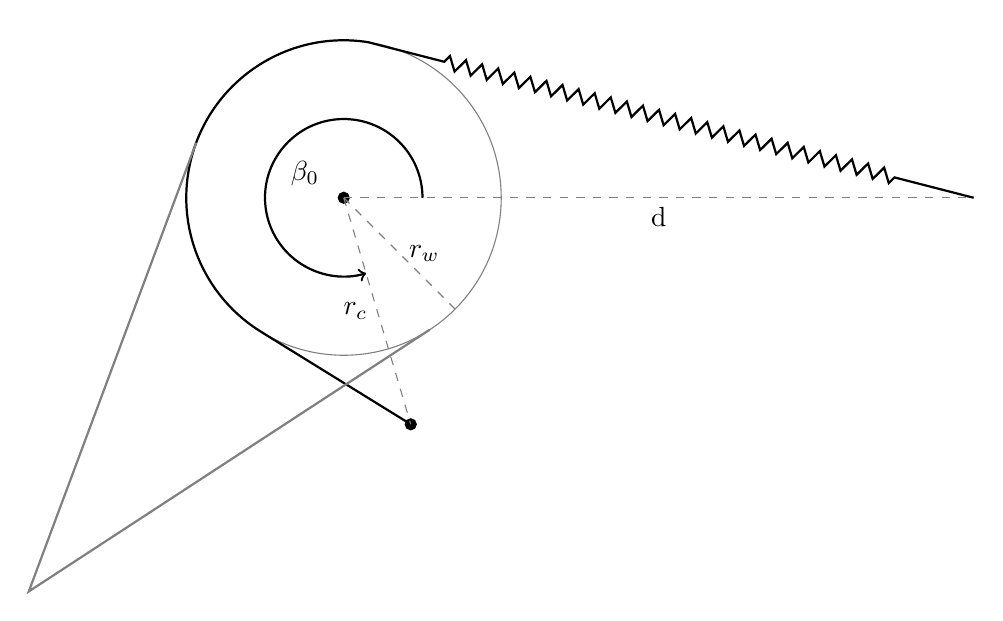
\begin{tikzpicture}
\tikzstyle{spring}=[thick,decorate,decoration={zigzag,pre length=1.0cm,post length=1.0cm,segment length=6}]
\filldraw[black] (0,0) circle (2pt); %origin
\draw[gray, dashed] (0,0) -- node[below, black] {d} (8,0) coordinate (ground);
\draw[gray] (0,0) circle (2);
\coordinate (tanone) at (0.3077, 1.9762);
\coordinate (tantwo) at (-1.05126,-1.70142);
\coordinate (ropecon) at (0.850987, -2.876773);
\filldraw[black] (ropecon) circle(2pt);
\draw[spring] (tanone) -- (ground);
\draw[black, thick] (tantwo) -- (ropecon);
\draw[gray, dashed] (0,0) -- node[left, black] {$r_c$} (ropecon);
\draw[black, thick, ->] (1,0) arc(0:286.48:1cm) node[midway, anchor=north west] {$\beta_0$};
\draw[black, thick] (tanone) arc(81.15:238.29:2cm); %makes clear that rope wraps around pulley
\draw[gray, dashed] (0,0) -- node[right, black] {$r_w$} (1.414, -1.414);
\draw[gray, thick] (-1.873845,0.699076) -- (-4,-5) -- (1.093357,-1.674685);
\end{tikzpicture}

\begin{description}
\item $r_w$: radius of the "winch" that drives the arm
\item $r_c$: distance from axis of rotation to connection point of the drive rope that wraps around the "winch"
\item $\beta$: angular distance arm would have to rotate in the throwing direction before the rope connection pointed toward the far end of the puller, with no rope left on the "winch". May be greater than one rotation, but $\beta_0 < 0$ will cause undefined behaviour.
\item $d$: same as in Configuration A
\end{description}
\subsubsection{Specifying Functions}
\textbf{All puller forces and torques are specified in contraction!} If using rubber, the force measured during the draw will be about twice as large as the force applied during the throw, due to hysteresis. Incorrectly using the draw force rather than the contraction force will cause serious inaccuracies in this case. Most other means of mechanical energy storage do not suffer from this problem.\par
In Configurations A and B, the dropdown "Force Parameters" menu lists the functions in CDT/custom\_functions/FofL.py. When a function is selected, its parameter names are used to generate the entries in the GUI. As such, the user can easily add custom functions simply by writing them in FofL.py, then restarting the GUI. Only parameters should be used (no args or kwargs), and it should be noted that all parameters passed from the GUI are strings. For the user unfamiliar with Python, the default options should suffice for most purposes.\par
When $R(\theta)$ and $F(\theta)$ or $\tau(\theta)$ and $R(\theta)$ are chosen to specify puller behaviour, the behaviour is analogous to that already explained for F(L). In the latter case, R is only needed to correctly calculate puller speed in postprocessing, and can otherwise be set to an arbitrary value.\par
The \emph{interpolate} function is available for all cases where a function needs to be specified. The text file it reads from should be located in CDT/custom\_functions. This file should have one data point per line, newline separated, with the format \verb|x<delimiter>f(x)|. The delimiter can be any character, but commas or spaces are most convenient. For example, if the delimiter was a comma, the file might contain the following:
\begin{lstlisting}
1.0,2000.0
1.5,2200.0
2.0,2500.0
\end{lstlisting}

\subsubsection{Interpolation Bounds}
Regardless of the method used for specifying forces, torques, or geometries, $\tau(\theta)$ is converted to the form discussed in \ref{Torque Source} before being passed to the dynamics solver. For most torque specification options, this entails finding a best fit to the desired torque profile. The interpolation bounds specify the range of arm angles over which the torque function should be fitted. The upper bound is automatically the initial value of $\theta$ (remember, $\theta$ should decrease during the throwing motion). The lower bound should be the lowest value of $\theta$ expected to be reached during the throwing motion. The simulation information window displays a warning if the guess of $\theta_{min}$ was wrong. The Calculate Fit button runs the interpolation and displays the result both visually and as text for the user's inspection. The Simulate button runs Calculate Fit automatically before starting the simulation.

\subsubsection{Hysteresis}
The reason for this parameter was discussed in \ref{Torque Source}. Calculate fit will work normally if it is omitted, but the simulation will fail. If unsure about the value and using any material other than rubber, set it to 1. For rubber, use 2. Remember that any direction dependent effects on the torque can \emph{only} be modeled using this parameter. 

\subsection{Simulation Types}
As discussed in section \ref{Simulation} there are only two core dynamics solvers. There are, however, many common use cases in the design process which are more complex than specifying the design parameters and getting a result. Typically, the user has some sort of goal for performance and constraints on what they can build. As such, various optimizing solvers are available to speed the search through the design space.
\subsubsection{Psi}
Use the dynamics solver directly by specifying the value of $\psi$ (the angle between the arm and the sling) at which the projectile is released. The dynamics solver finds the time where $\psi = \psi_{target}$ and returns the state vector at that time.
\subsubsection{Launch Angle}
Stop the simulation when the projectile velocity vector reaches a specified angle AND the projectile is no longer resting on the platform AND $\psi_{min} < \psi < \psi_{max}$. The angle convention is intuitive - 0 corresponds to throwing straight forward, $\pi/4$ corresponds to throwing forward at a 45\degree angle. Watch the animation to detect potentially wonky behaviour in machines that complete multiple rotations before throwing.
\subsubsection{Sling Length Optimizer}
Same as Launch Angle, except sling length is varied within specified limits such that the arm reaches a specified target angle at the time the projectile is released. Note that the convention for arm angle here is the same as the one shown in section \ref{Dynamics Assembly Parameters}. Should run in less than ten seconds on most machines.
\subsubsection{Arm Inertia Optimizer}
Same as Sling Length Optimizer, but varies arm inertia instead.
\subsubsection{Max Speed}
Given targets for final arm angle and launch angle, and limits on arm inertia, sling length, and release angle, finds the configuration that produces the maximum throw speed. If the limits are set appropriately, this should occur when the arm stalls at the same time the projectile releases. May take a minute or more to run on slower machines, so be sure to set the solver timeout appropriately.

\subsection{Postprocessing}
The two plot windows at the bottom of the interface can display most relevant information about the performance of the machine after the simulation is complete. The one on the right handles the "normal" plotting functions, where x and y axis data can be set independently. The one on the left handles more specialized features, like animation and loading states of the arm.
\subsubsection{Puller Speed} Available on the right-side plot. It is important to note that the speed is \emph{negative} if the puller is \emph{contracting}. Puller speed cannot be calculated correctly if $R(\theta)$ is not physically accurate.
\subsubsection{Animation} A "stick figure" representation of the throwing motion. Accidentally hitting the Play button while the animation is already playing causes strange but harmless behaviour.
\subsubsection{Arm Load} Used to display and optionally save the arm loading state. The text file generated is for evenly spaced points in time, and has the format:\\ \verb|<time> <tip force x> <tip force y> <ang. speed> <ang.accel.>|\\
Refer to the arm tip coordinate frame in \ref{Dynamics Assembly Parameters} for direction of the tip forces. Arm angular speed is $>0$ if the arm in moving in the throwing direction (clockwise on the diagram), and arm angular acceleration is positive when accelerating in this direction.
\subsubsection{Projectile Path} Saves the path taken by the projectile. Useful for ensuring structural members and triggers don't get hit. Format is \verb|x y z|, where $z=0$ and the other entries are in the base frame. The format can be directly imported to Solidworks. The scale factor option simply multiplies all entries by the entered value to change units.
\subsubsection{Efficiency} There are several ways to talk about the energy efficiency of a catapult, but the most useful for design purposes in many cases is to compare the energies of the arm and the sling+projectile system. The energy considered here is the sum of gravitational potential and kinetic, relative to the base frame.
\subsubsection{Puller Potential Energy} This tool allows finding the overall energy efficiency of the system, from puller to projectile, and is somewhat more difficult to use. It finds the zeroes of the torque function in the the domain $\theta < \theta_0$, prunes the zeroes that are not candidates for minima of the integral, then selects the zero corresponding to the largest potential energy drop relative to the initial condition. The difficulty is that, since the torque it uses is the polynomial fit to the actual torque, and even the actual torque may be a convenient approximation, the values it returns may be unexpected and useless, as they correspond to artifacts of the fit or approximation rather than physical reality. This can usually be fixed either by changing interpolation range in the torque specification, or using the "Direct" option for specifying $\tau(\theta)$. Note that the plot cannot be updated until the simulation is run again. The red dots mark zeroes of the torque function, and the black dot marks the initial condition.
\subsubsection{Axle Reaction Force} In some higher performance catapults, the entire machine may be thrown by the unbalanced force on the axle as the arm rotates. This plotting tool is useful for design of hold-downs to prevent unwanted motion of the machine during a throw. The forces given are the loads on the axle in the base frame. For example, a y-direction force of +100 would tend to pull the whole machine up.

\section{Arm Design Hardness}
 At the higher performance levels, by far the most difficult problem is constructing the arm to be sufficiently strong without an excessively high rotational inertia. The arm design hardness (denoted here as $\mathcal{H}$) is a powerful tool when choosing between catapult designs, as it provides a single number to compare design difficulties. Solving a more difficult design problem entails either better materials or more complex geometry. All solver options return the calculated $\mathcal{H}$ value in the output. Due to the various approximations involved in calculating $\mathcal{H}$, one should not read too much into the exact values, or choose between designs based on a small difference in values. It is, however, a good measure of the general feasibility of constructing a design. 500 is easy, 2000 requires only basic competency. I've successfully designed an arm with $\mathcal{H}=35000$, though at this point one is well into the realm of exotic materials and intricate geometry. The process of determining $\mathcal{H}$ also entailed quantifying the material property corresponding to suitability for arm design. This value, denoted $\mathcal{A}$, is approximately determined by
 \[\mathcal{A} = E^{0.279} \sigma_y^{0.721} \rho^{-1.606}\]
 The strong dependence on $\rho$ has some interesting effects - for example, most common woods are superior to 6Al4V titanium alloy! However, one must remember that this only holds for a given geometry - as titanium is isotropic, and can be formed by casting or 3d printing, the disadvantage in material suitability can be countered by employing more highly optimized shapes.

\section{Units}
No units of measure (seconds, pounds, hogsheads of mercury per cubic furlong, etc) are used anywhere in the CDT. The user is free to use whatever system they please, so long as it is consistent. If you don't know what a consistent unit system is, defaulting to MKS is probably easiest.
\section{Troubleshooting}
The only "mysterious" errors observed in testing of the CDT occurred when the dynamics solver manager was having trouble determining the time of transition between platform and free dynamics, when simulating a mechanism with an unusually short timescale. If the solver appears to fail to finish for reasons unrelated to optimization bounds, and the total length of the simulation is less than 0.01 or so, this may be the problem. It can be resolved by modifying transition\_tolerance in dyn\_full\_platform to a larger value. Don't forget to change it back afterward! Although it has not be seen to cause failures, termination\_tolerance in dyn\_full\_simple could theoretically cause a similar issue, and can be modified as well if needed. Both these functions are located in CDT/CDTtools/dyn\_core\_tools.py. Alternatively, the timescale could be increased by changing the units. Make sure to keep your units consistent!
\subsubsection{Logs}
While most errors will appear in a window directly in the GUI, a few quiet failures are possible involving the backend code. Check CDT/logfile after quitting the GUI to see if any errors were recorded.

\end{document}
